\chapter{整机调试问题记录}
\label{cha:Debug}

\section{待机状态下电机发热}

2020年4月12日下午三点多在调试小车运动的时候,使用了如下代码在PCBv2上进行了测试:

\inputminted[mathescape, linenos, breaklines]{c}{Code/Stepper-3-Movement/Stepper-3-Movement.ino}

连上电池、烧写程序、等待五秒后两电机经过加减速过程反向转动10000 Step后停止。

% ,推动小车向前运动一段距离。

但是在电机停止后我没有像往常一样拔下锂电池,大约十分钟,我闻到了金属加热后表面涂层的焦糊气味(有点像电弧焊的气味),寻找来源的过程中感受到了小车的热辐射,第一反应就是把锂电池拔下来,感受到锂电并没有发热松了一口气,大致判定是电机发热,我做了一个错误决定,用手指伸到了电机外壳上验证是不是电机在发热,感受到电机温度应该在200-300摄氏度之间,手指被烫伤。

怀疑是Speed=0时AccelStepper库依然在向DRV8825发送比较低频的PWM信号,使得有大电流持续通过电机绕组。

目前3D打印的小车底盘已经部分融化变形(熔点150摄氏度),如图~\ref{fig:DebugHeat}。

% 如果我碰巧离开工位,温度会继续上升,可能会引发火灾。

\begin{figure}[htbp]
    \centering
    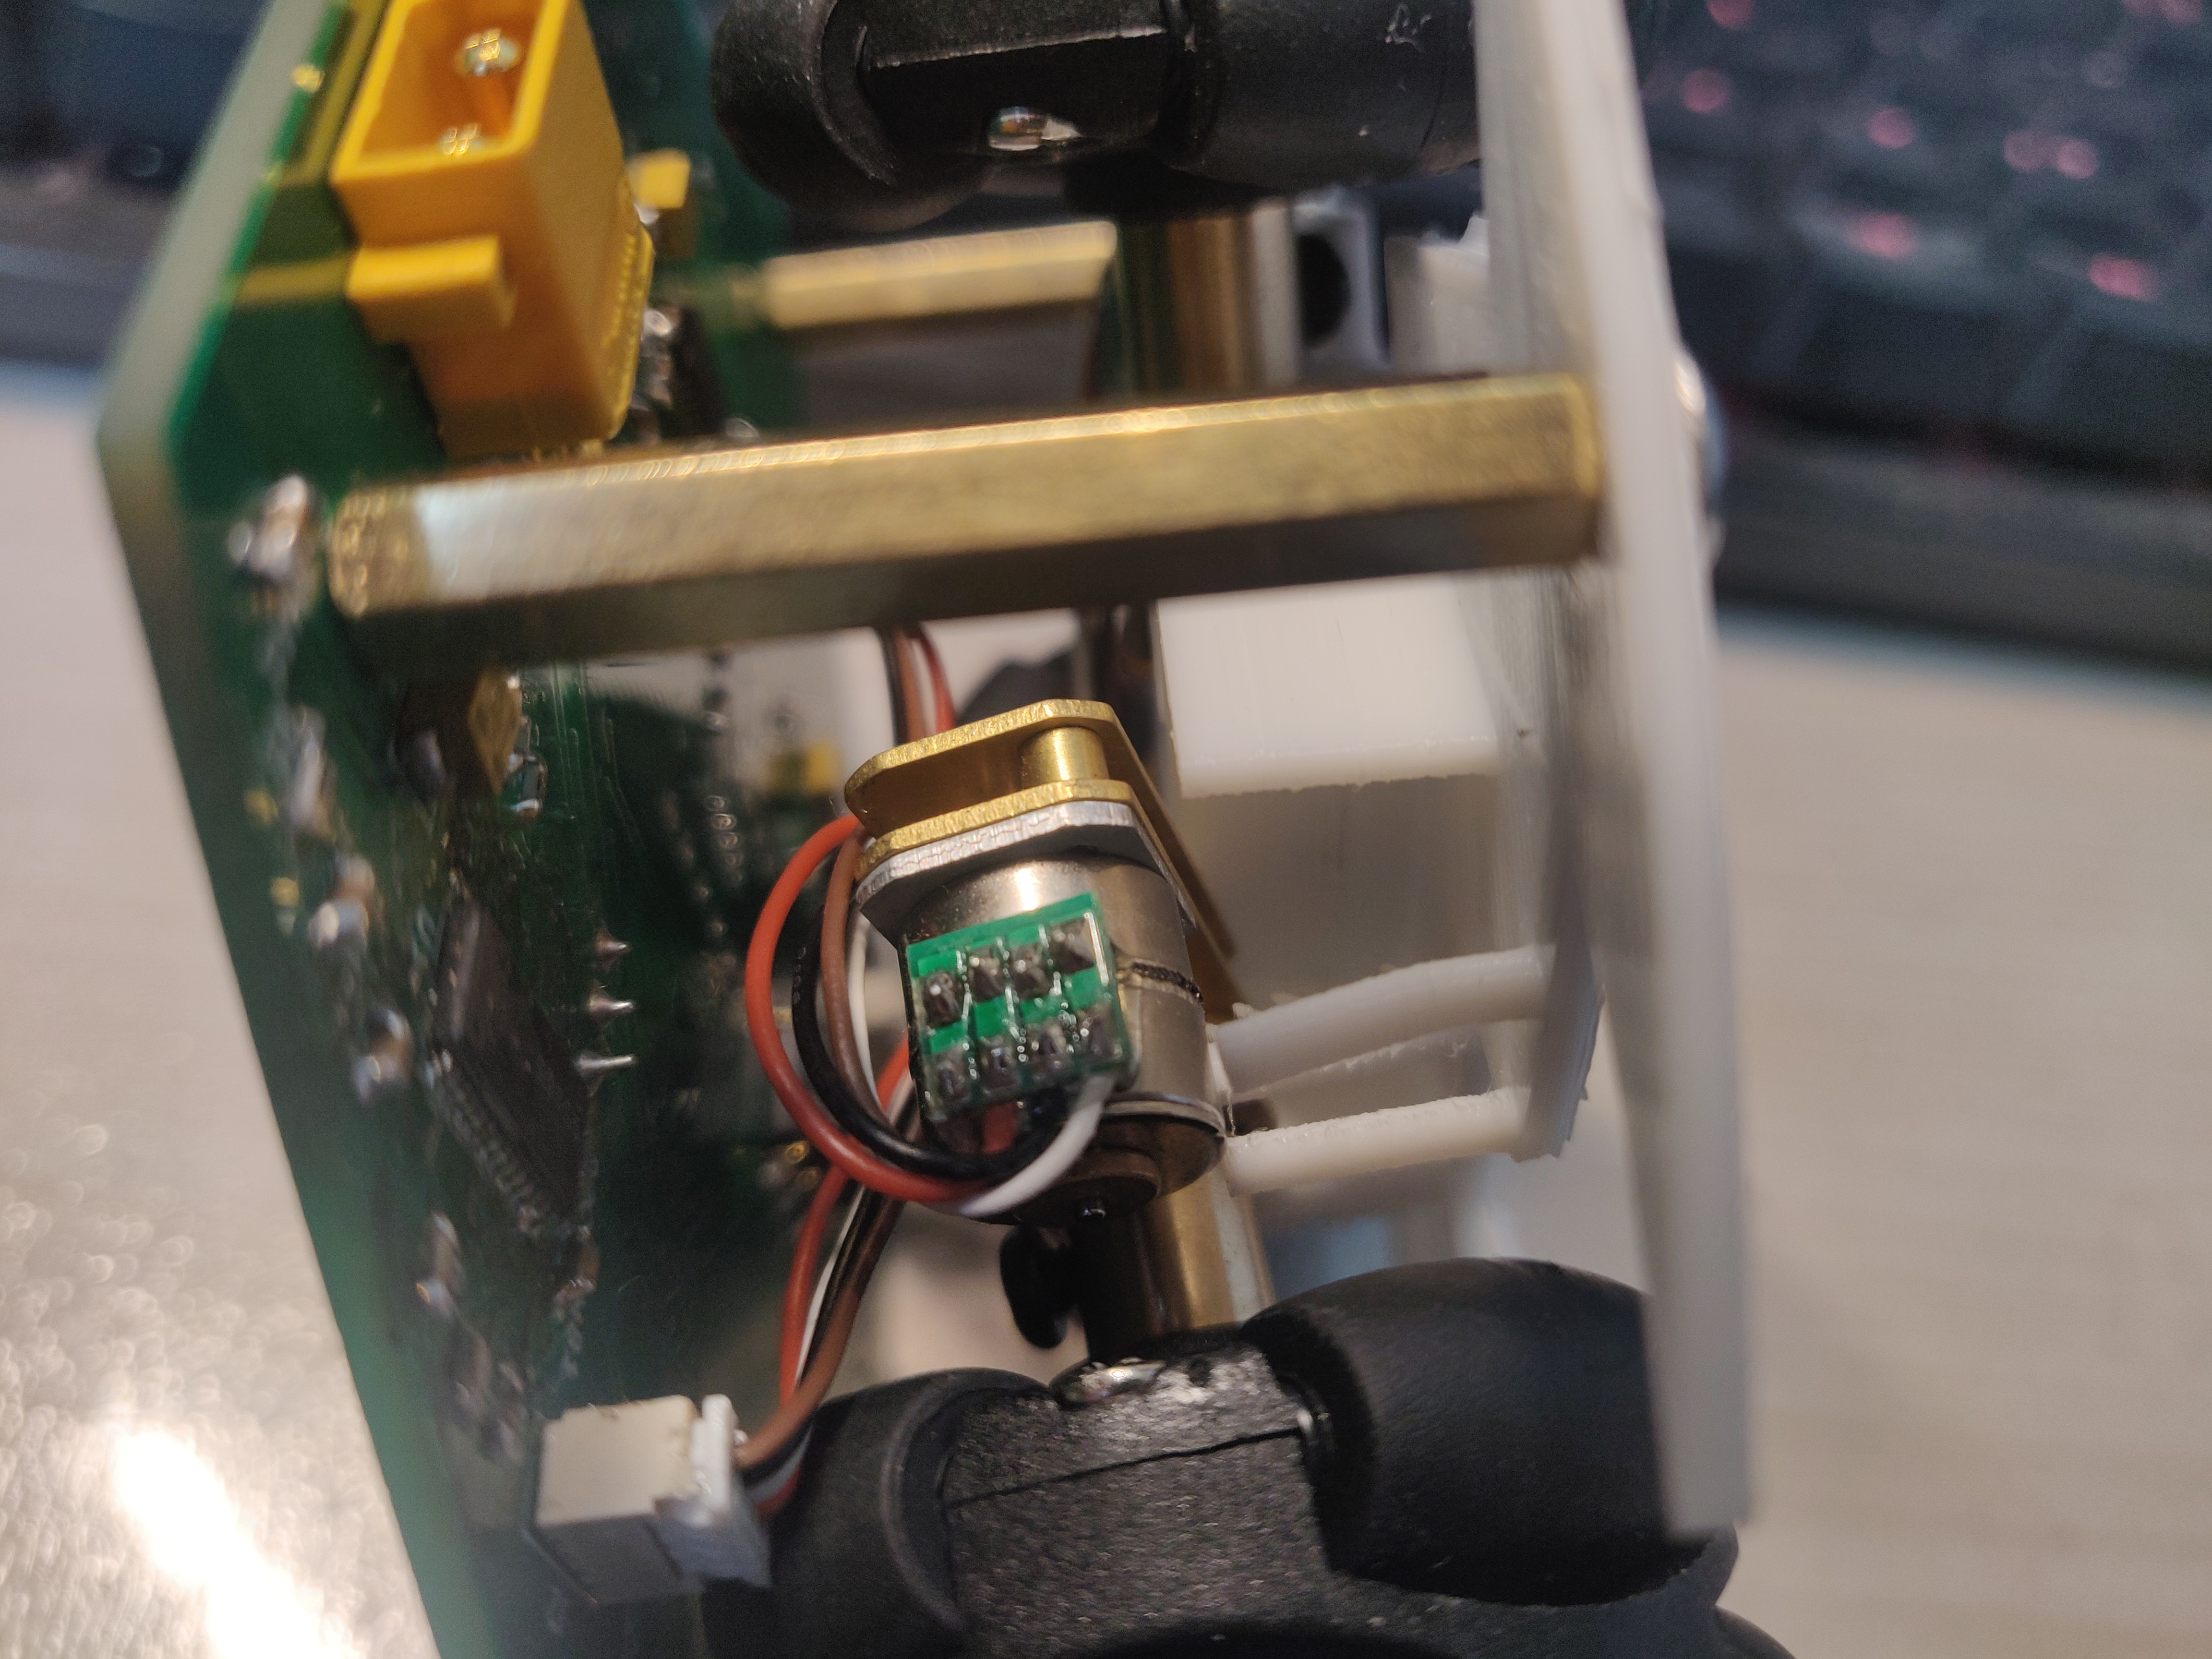
\includegraphics[width=\columnwidth]{DebugHeat.jpg}
    \caption{融化变形的PLA电机固定}
    \label{fig:DebugHeat}
\end{figure}

得到以下经验教训:

\begin{enumerate}
    \item 将来调试完成后立即断开锂电的连接,同时调试时间也控制在一分钟以内以减少发热量。
    \item 购买二氧化碳灭火器放在工位旁以防万一。
    \item 感受到热浪和焦糊味要保持清醒头脑,不要贸然触碰可能的发热点。
\end{enumerate}


\section{时钟问题}

时钟周期比我代码设定的长了16倍,原因未知。

% 测试代码如下:

% \inputminted[mathescape, linenos, breaklines]{c}{Code/PWM-Test/PWM-Test.ino}

测得波形数据如图~\ref{fig:DebugClock}。

\begin{figure}[htbp]
    \centering
    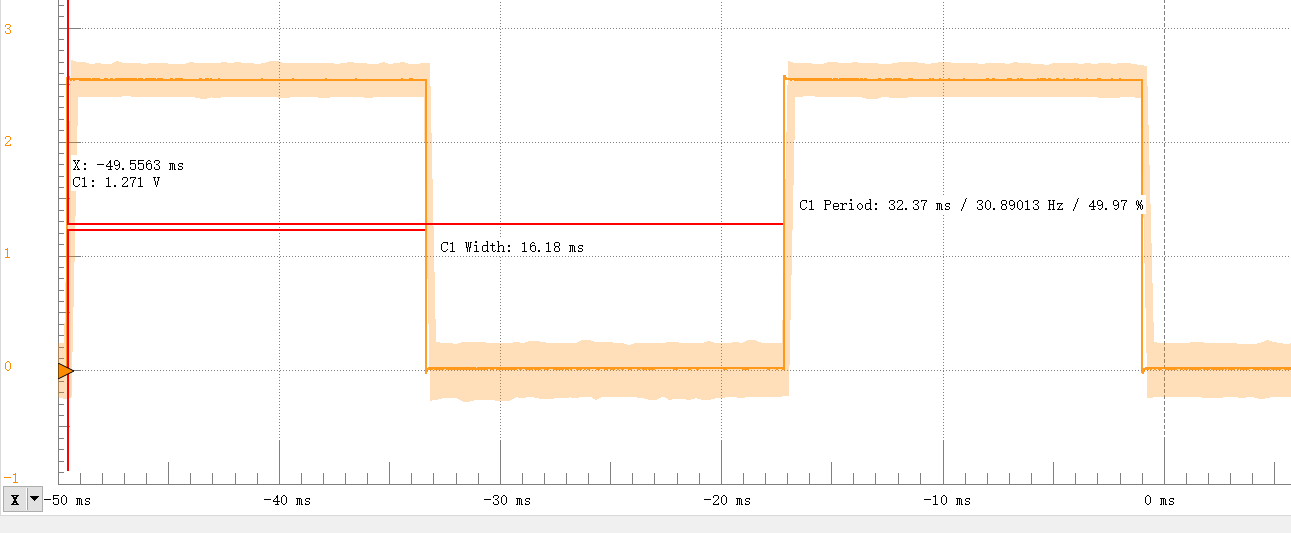
\includegraphics[width=\columnwidth]{DebugClock.png}
    \caption{实测时钟周期}
    \label{fig:DebugClock}
\end{figure}

目前是在我代码里面设定一个TimeScale为16来暂时解决。但感觉电机转动还是慢,不知道是不是我用的AVR的问题

\section{电机不转解决方案}

更换电机,排除电机本身问题:有一次是电机联轴器螺丝太长,卡在底盘上了。

使用锂电池或足功率的开关电源,曾经用充电宝开关电源供电不足以三个电机一起转,出现接上三个反而总功耗比两个小的情况,以及电机发出轻微的吱吱声。

检查Mega2560信号输出到DRV8825 STEP和DIR引脚回路,MCU是否输出PWM波。

检查3.3V分压回路是否按照3:5分压,即设定额定电流值。

检查DRV8825输出是否有密集的方波。如果有方波却转不了,也遇到过,问题未知,但之后那个8825就不输出波形了,可能是我测试的时候烧坏了
也有可能是接触不良。

用示波器对比不同DRV8825各引脚电压值,分析问题。

如果输入正常,没有输出,可能是DRV8825焊接问题,注意看焊盘有没有和引脚良好接触,

也很有可能是DRV8825坏了,需要使用堆锡后烙铁头左右横跳拆下来8825,并注意清理Thermal Via上面的锡(热风枪+吸锡器/刀头烙铁往旁边焊盘上拨,和清理连锡操作差不多,简单很多),其实很常见,基本每三个就有一个有问题,不知道是不是我从立创商城买的质量不好(后来发现并不是)。

气,2020/4/22搞了一整天,换下来三片芯片,如图~\ref{fig:DebugDRV8825}。最后发现三个驱动轮流不输出,最后发现是电池没电了。。。

\begin{figure}[htbp]
    \centering
    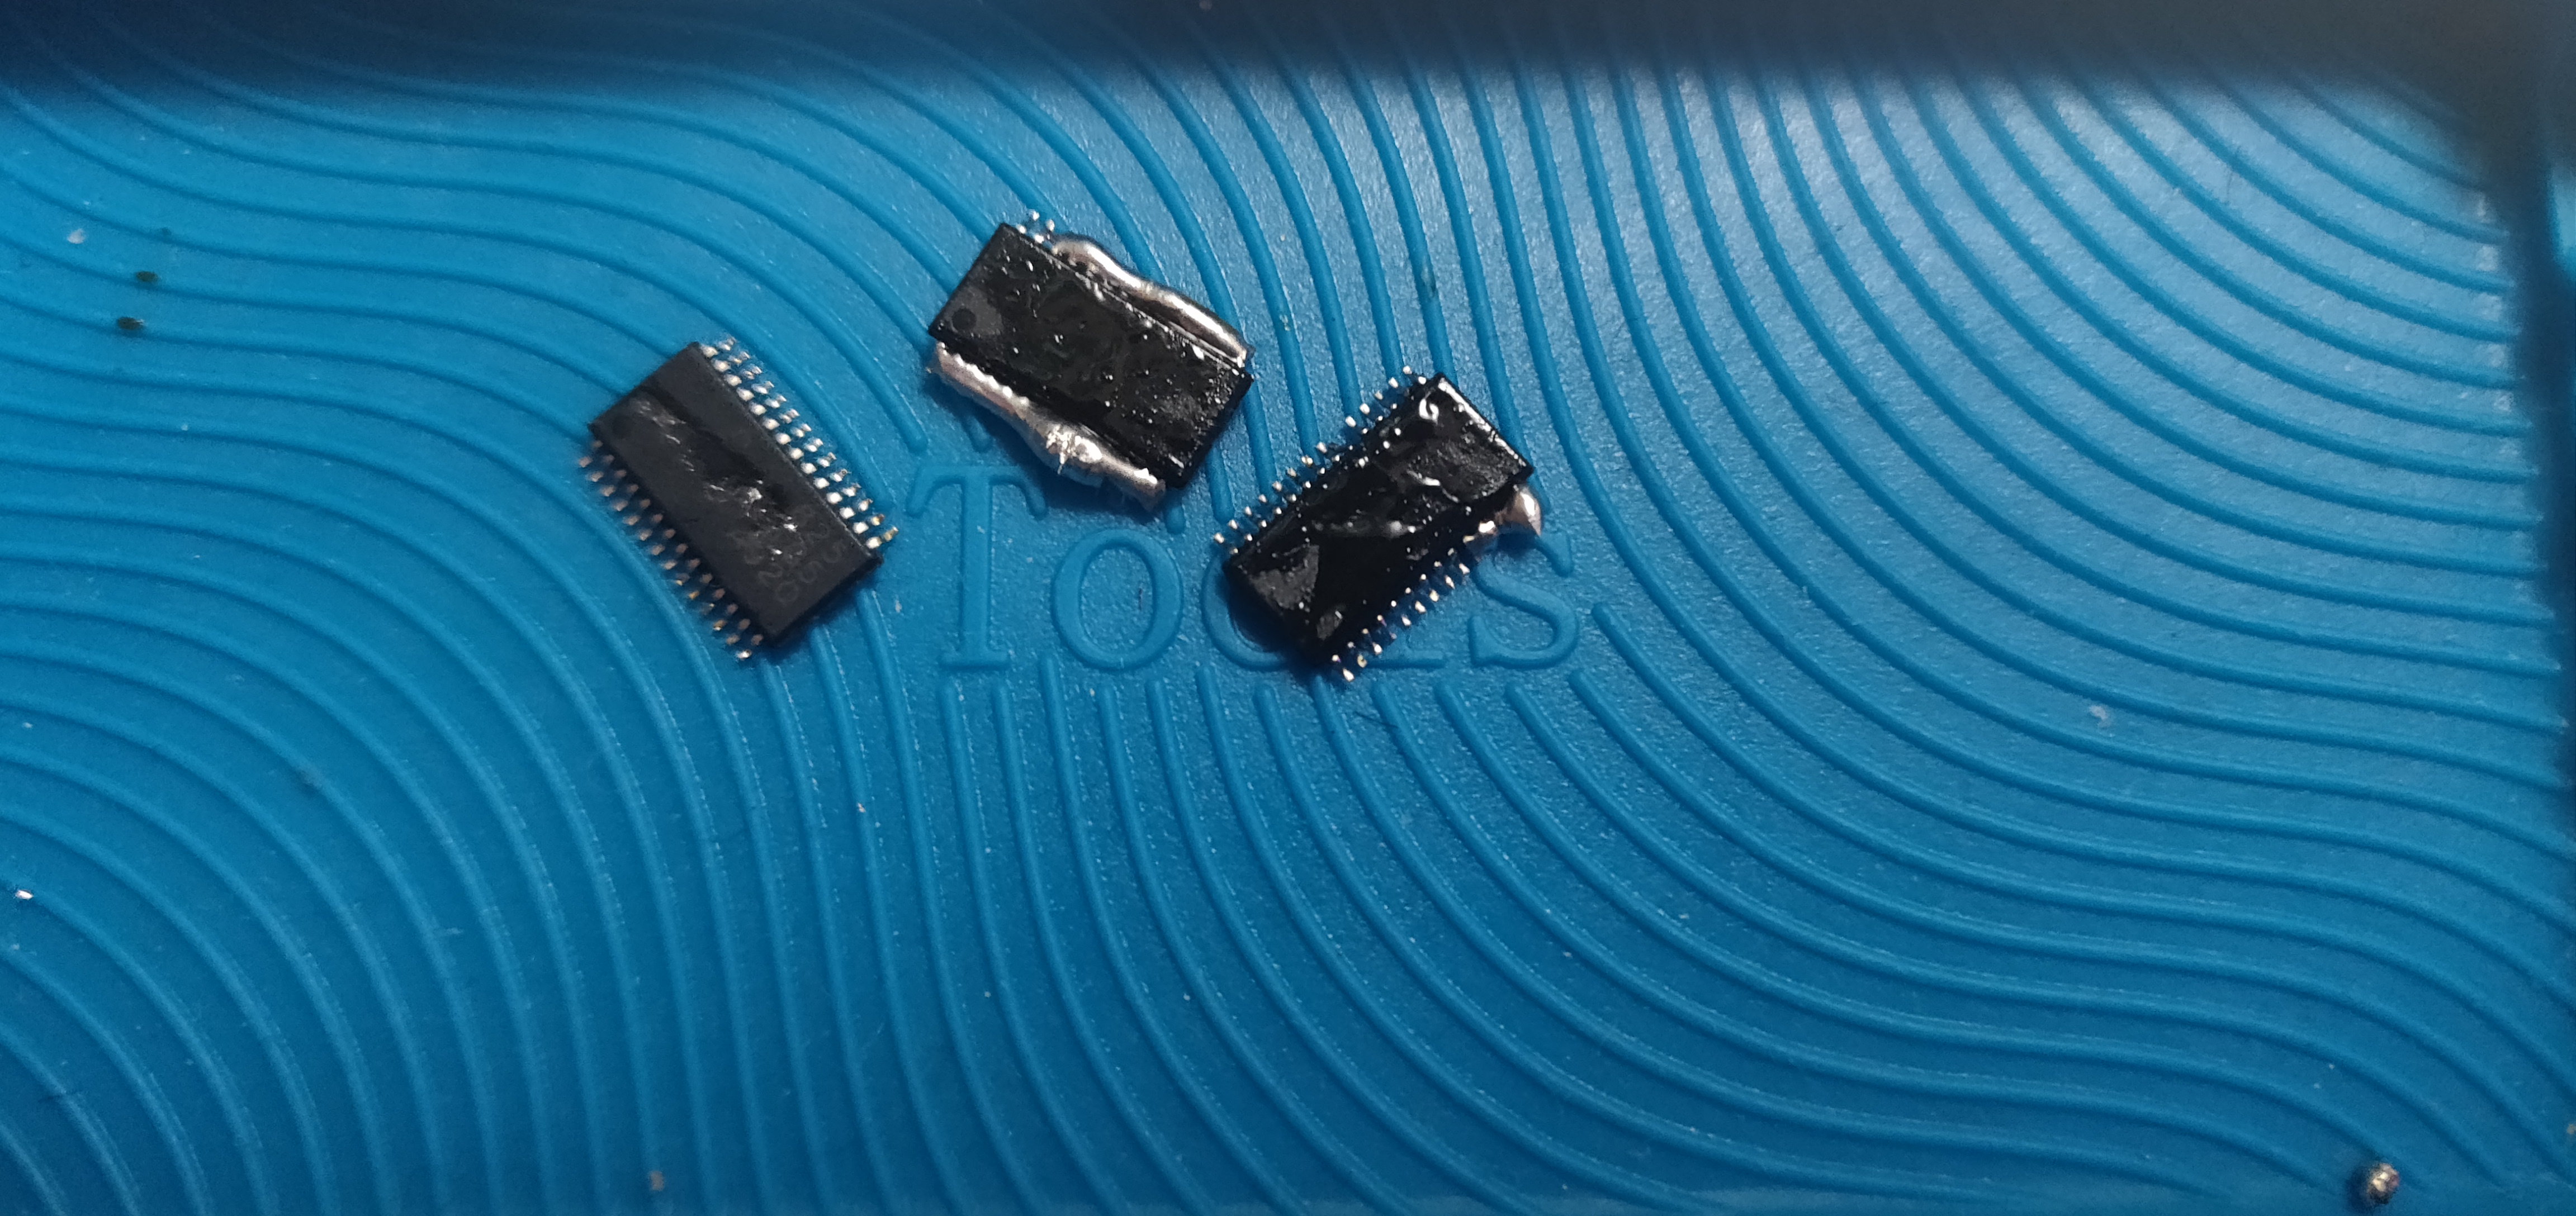
\includegraphics[width=\columnwidth]{DebugDRV8825.jpg}
    \caption{误以为芯片问题而换下来的三片芯片}
    \label{fig:DebugDRV8825}
\end{figure}

使用的2S锂电池额定电压为7.4V,充满电能到8V以上,用一段时间就会跌到7V左右,这时候电压会不足以驱动DRV8825,所以随着电池电压的升高降低出现时好时坏的情况。

当即购买了3S的锂电,11.2V的额定电压足以驱动DRV8825。

2020/4/22遇到了一个确定质量问题的DRV8825,正常的两片输出波形如图~\ref{fig:DRV8825DebugCorrectOutput},但是这片DRV8825输出波形如图~\ref{fig:DRV8825DebugErrorOutput},全桥有一路坏了导致半个周期短路,其发热也十分剧烈,拿着覆铜都能感受到烫。此时及时断电更换为正确做法。

\begin{figure}[htbp]
    \centering
    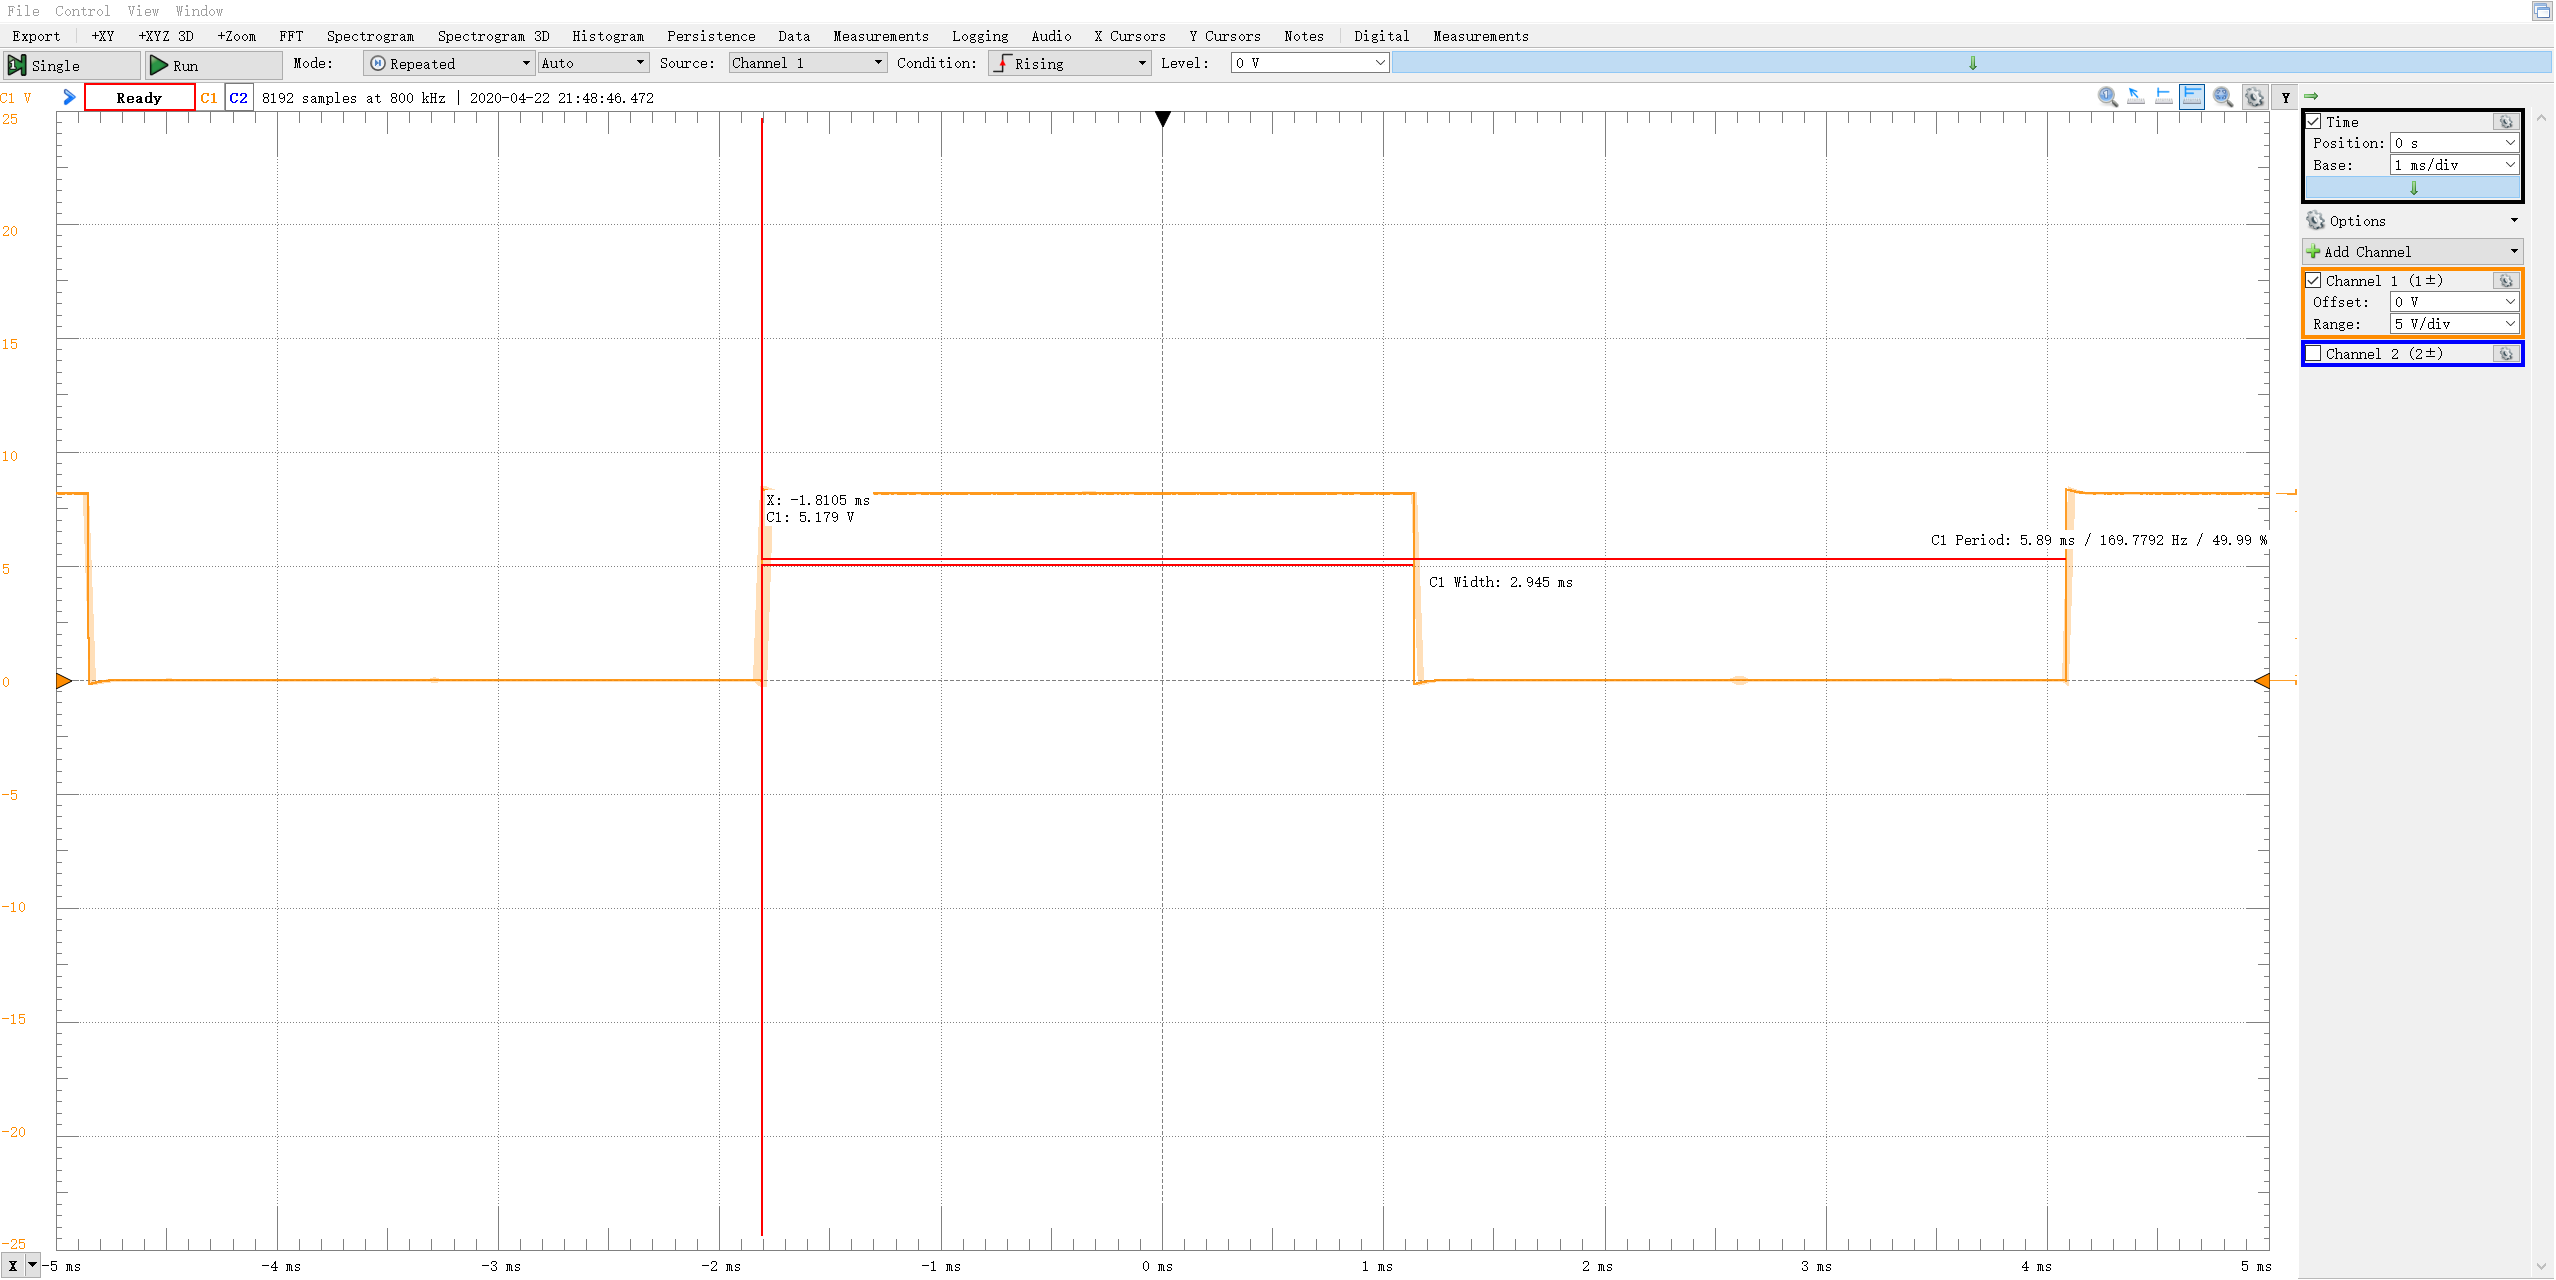
\includegraphics[width=\columnwidth]{DRV8825DebugCorrectOutput.png}
    \caption{正常的DRV8825输出波形}
    \label{fig:DRV8825DebugCorrectOutput}
\end{figure}

\begin{figure}[htbp]
    \centering
    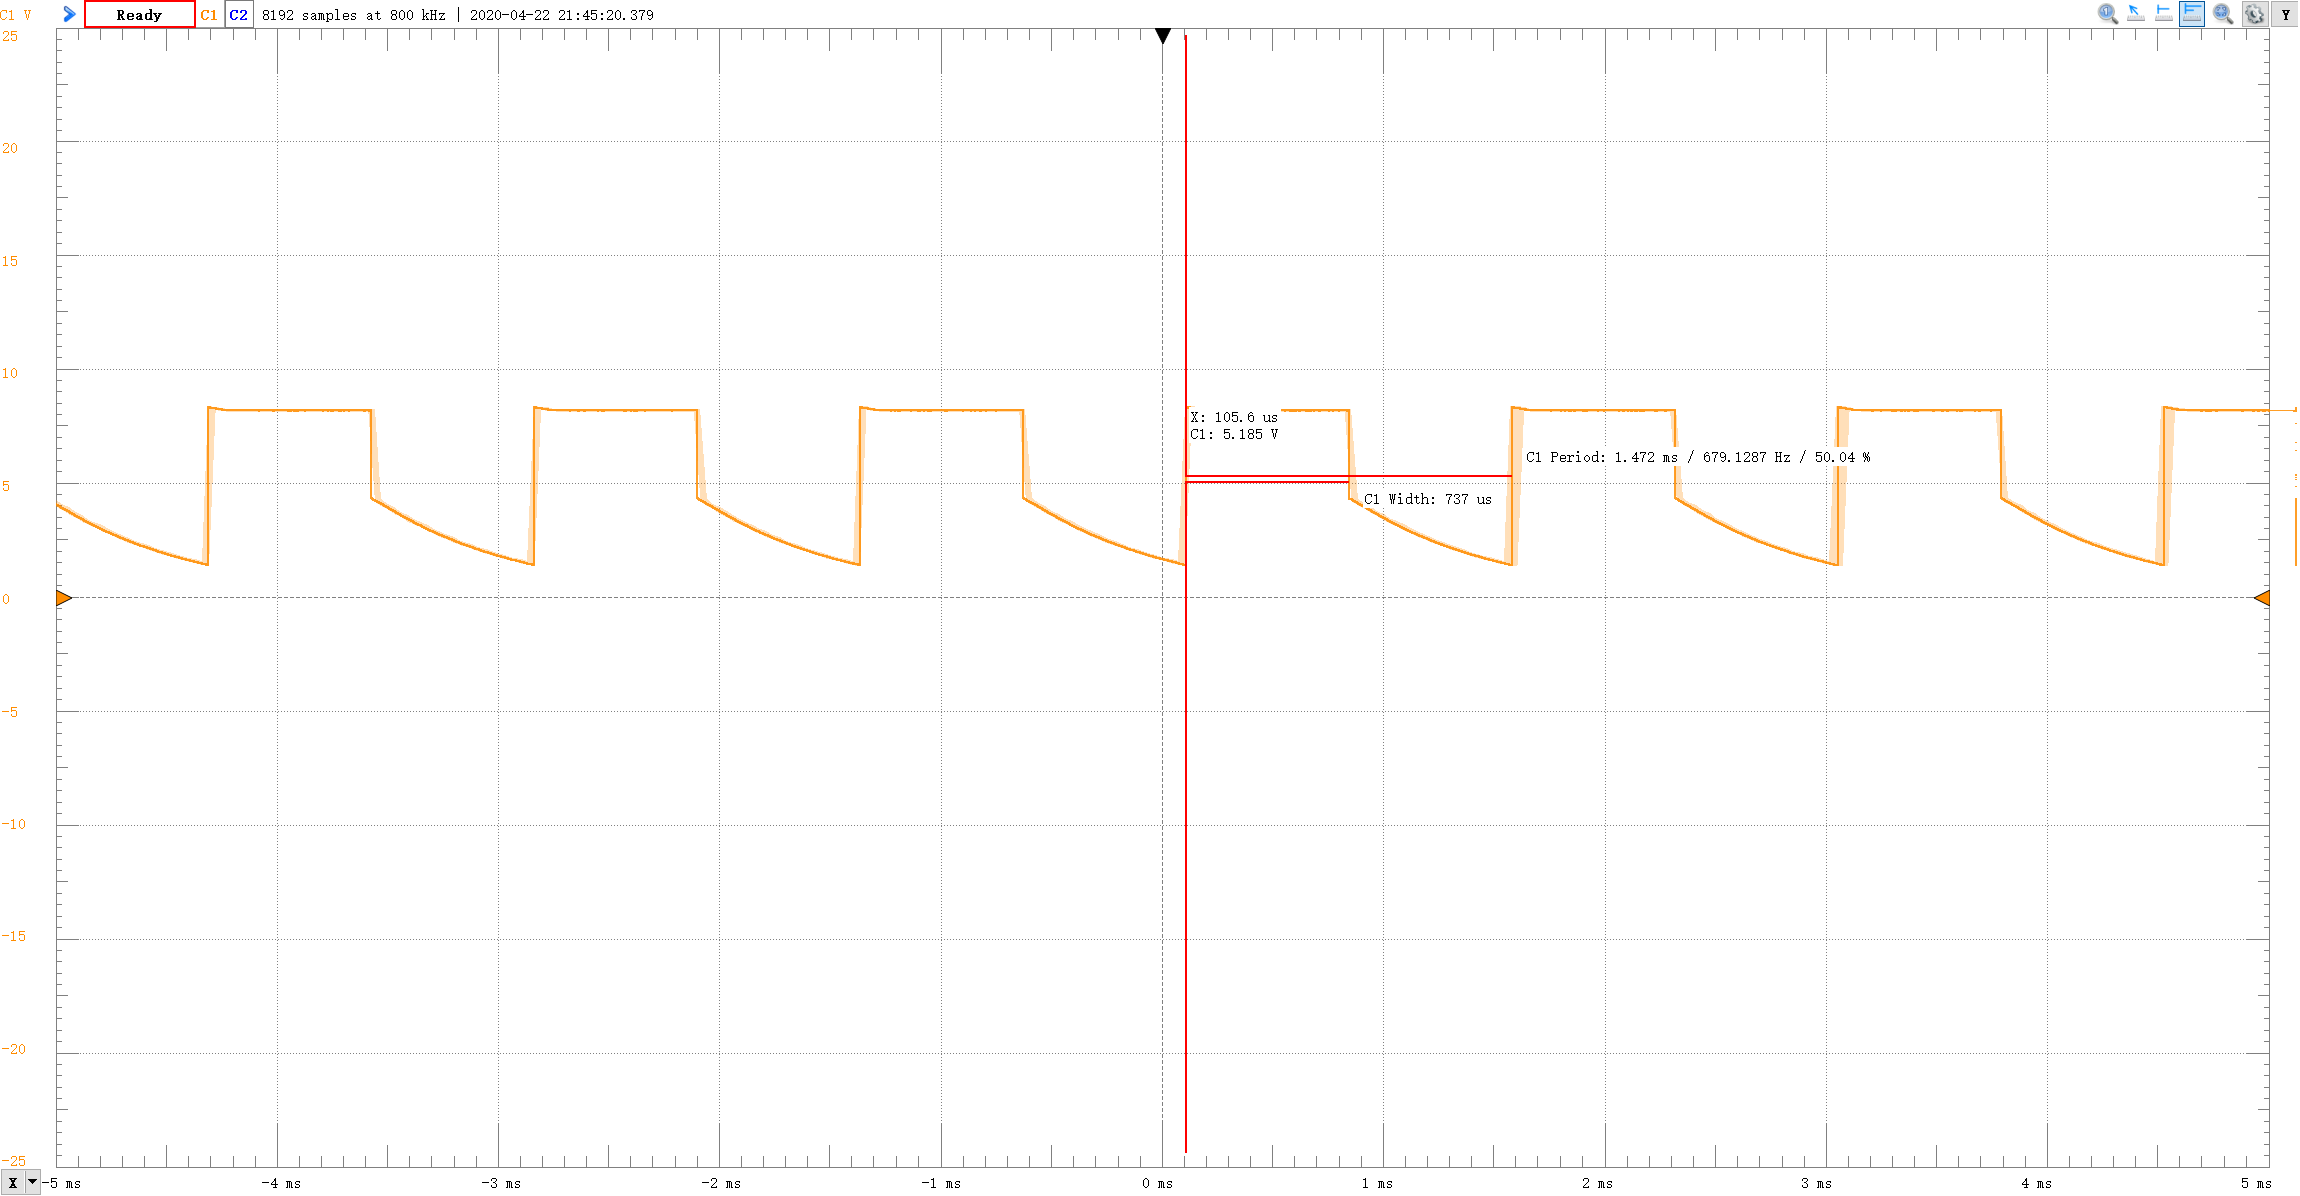
\includegraphics[width=\columnwidth]{DRV8825DebugErrorOutput.png}
    \caption{有问题的DRV8825输出波形}
    \label{fig:DRV8825DebugErrorOutput}
\end{figure}


\section{其他问题}

V3.1版本的PCB一共做了5块,一个炸了钽电容,如图~\ref{fig:DebugCapacitor0}(原因不明,我在仔细查,但是不太敢贸然上电,去掉炸的电容后功率表测试空载功率远超正常板,如图~\ref{fig:DebugCapacitor}),去掉全部锂电容和电解电容并除去了几处连锡好了。

\begin{figure}[htbp]
    \centering
    \includegraphics[width=\columnwidth]{DebugCapacitor0.jpg}
    \caption{炸了电容的板子}
    \label{fig:DebugCapacitor0}
\end{figure}

\begin{figure}[htbp]
    \centering
    \includegraphics[width=\columnwidth]{DebugCapacitor.jpg}
    \caption{去掉炸的电容后的板子}
    \label{fig:DebugCapacitor}
\end{figure}

2020年4月26日测试新买来的3S锂电池(标称电压11.2V,实际刚充满电电压12.4V)时,炸了第二个钽电容,如图~\ref{fig:DebugCapacitor1},这时我才想起来查看购买的钽电容的型号和耐压值,如图~\ref{fig:DebugCapacitor2}。发现是6.3V,其实电容上面也标明了,如图~\ref{fig:DebugCapacitor3},我加上的电压12V已经远超耐压。于是把全部钽电容焊下来,防止未来再炸电容。

\begin{figure}[htbp]
    \centering
    \includegraphics[width=\columnwidth]{DebugCapacitor1.jpg}
    \caption{炸了电容的第二块板}
    \label{fig:DebugCapacitor1}
\end{figure}

\begin{figure}[htbp]
    \centering
    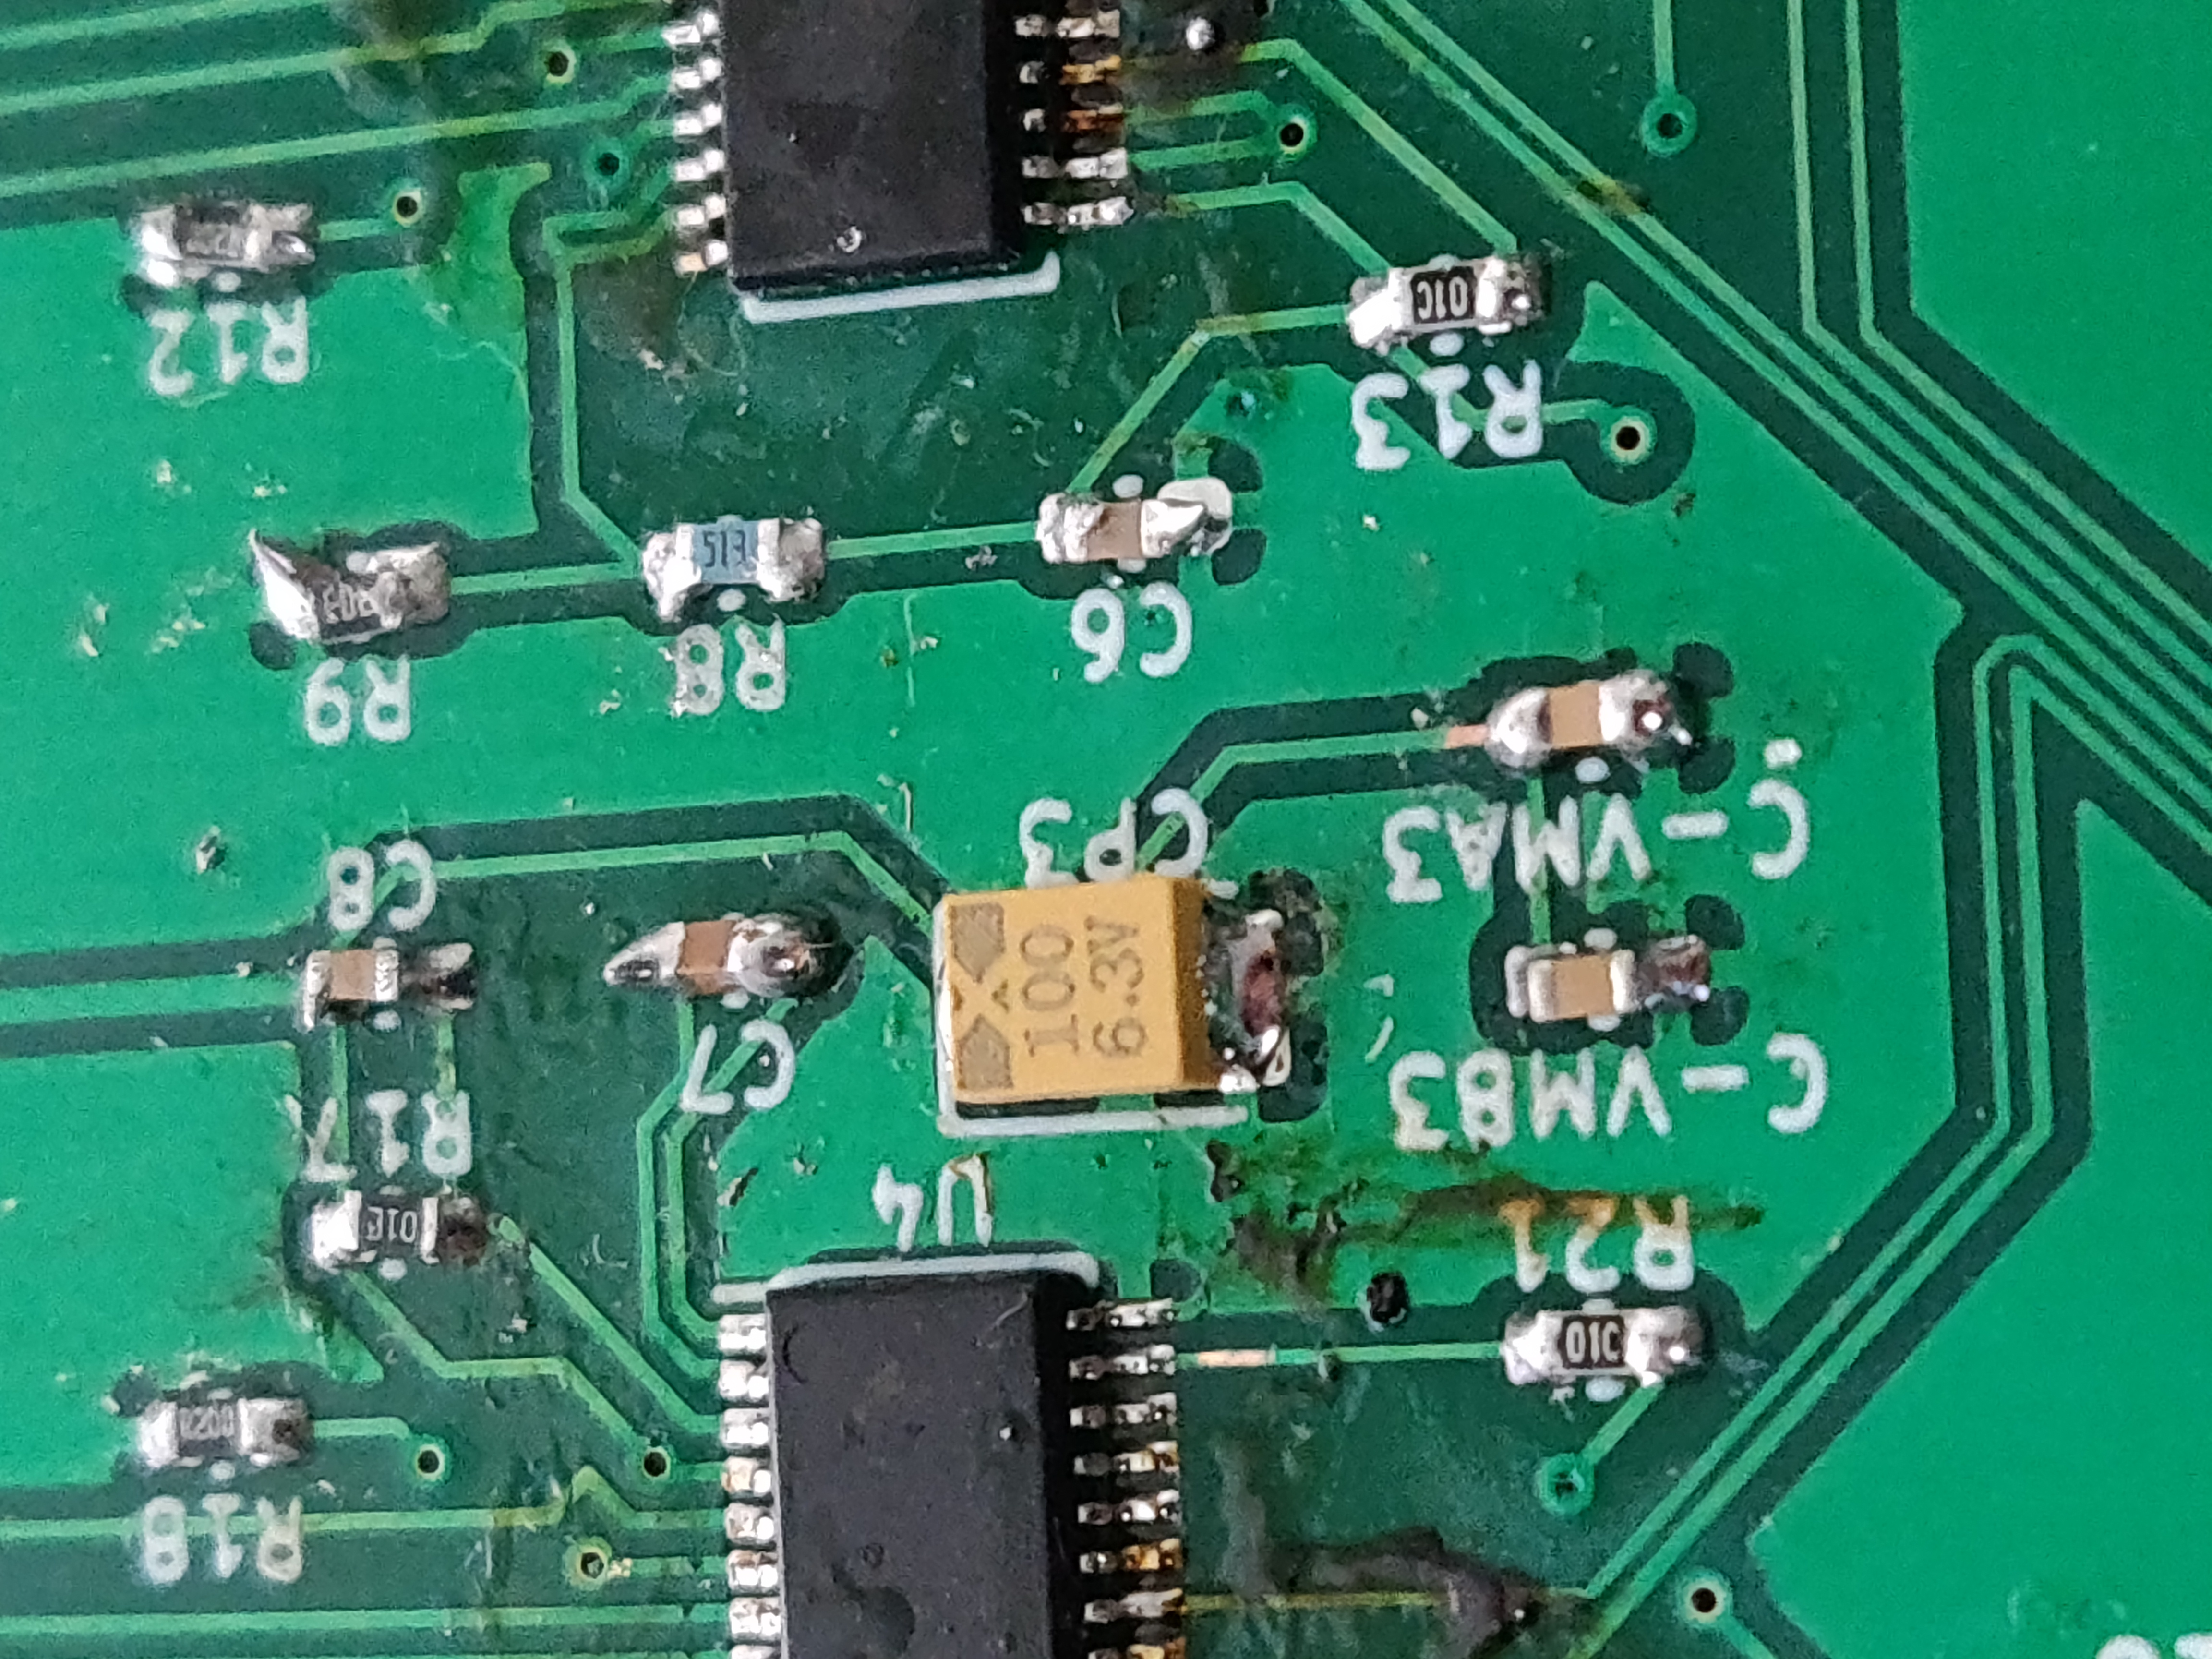
\includegraphics[width=\columnwidth]{DebugCapacitor2.jpg}
    \caption{电容上的标识}
    \label{fig:DebugCapacitor2}
\end{figure}

\begin{figure}[htbp]
    \centering
    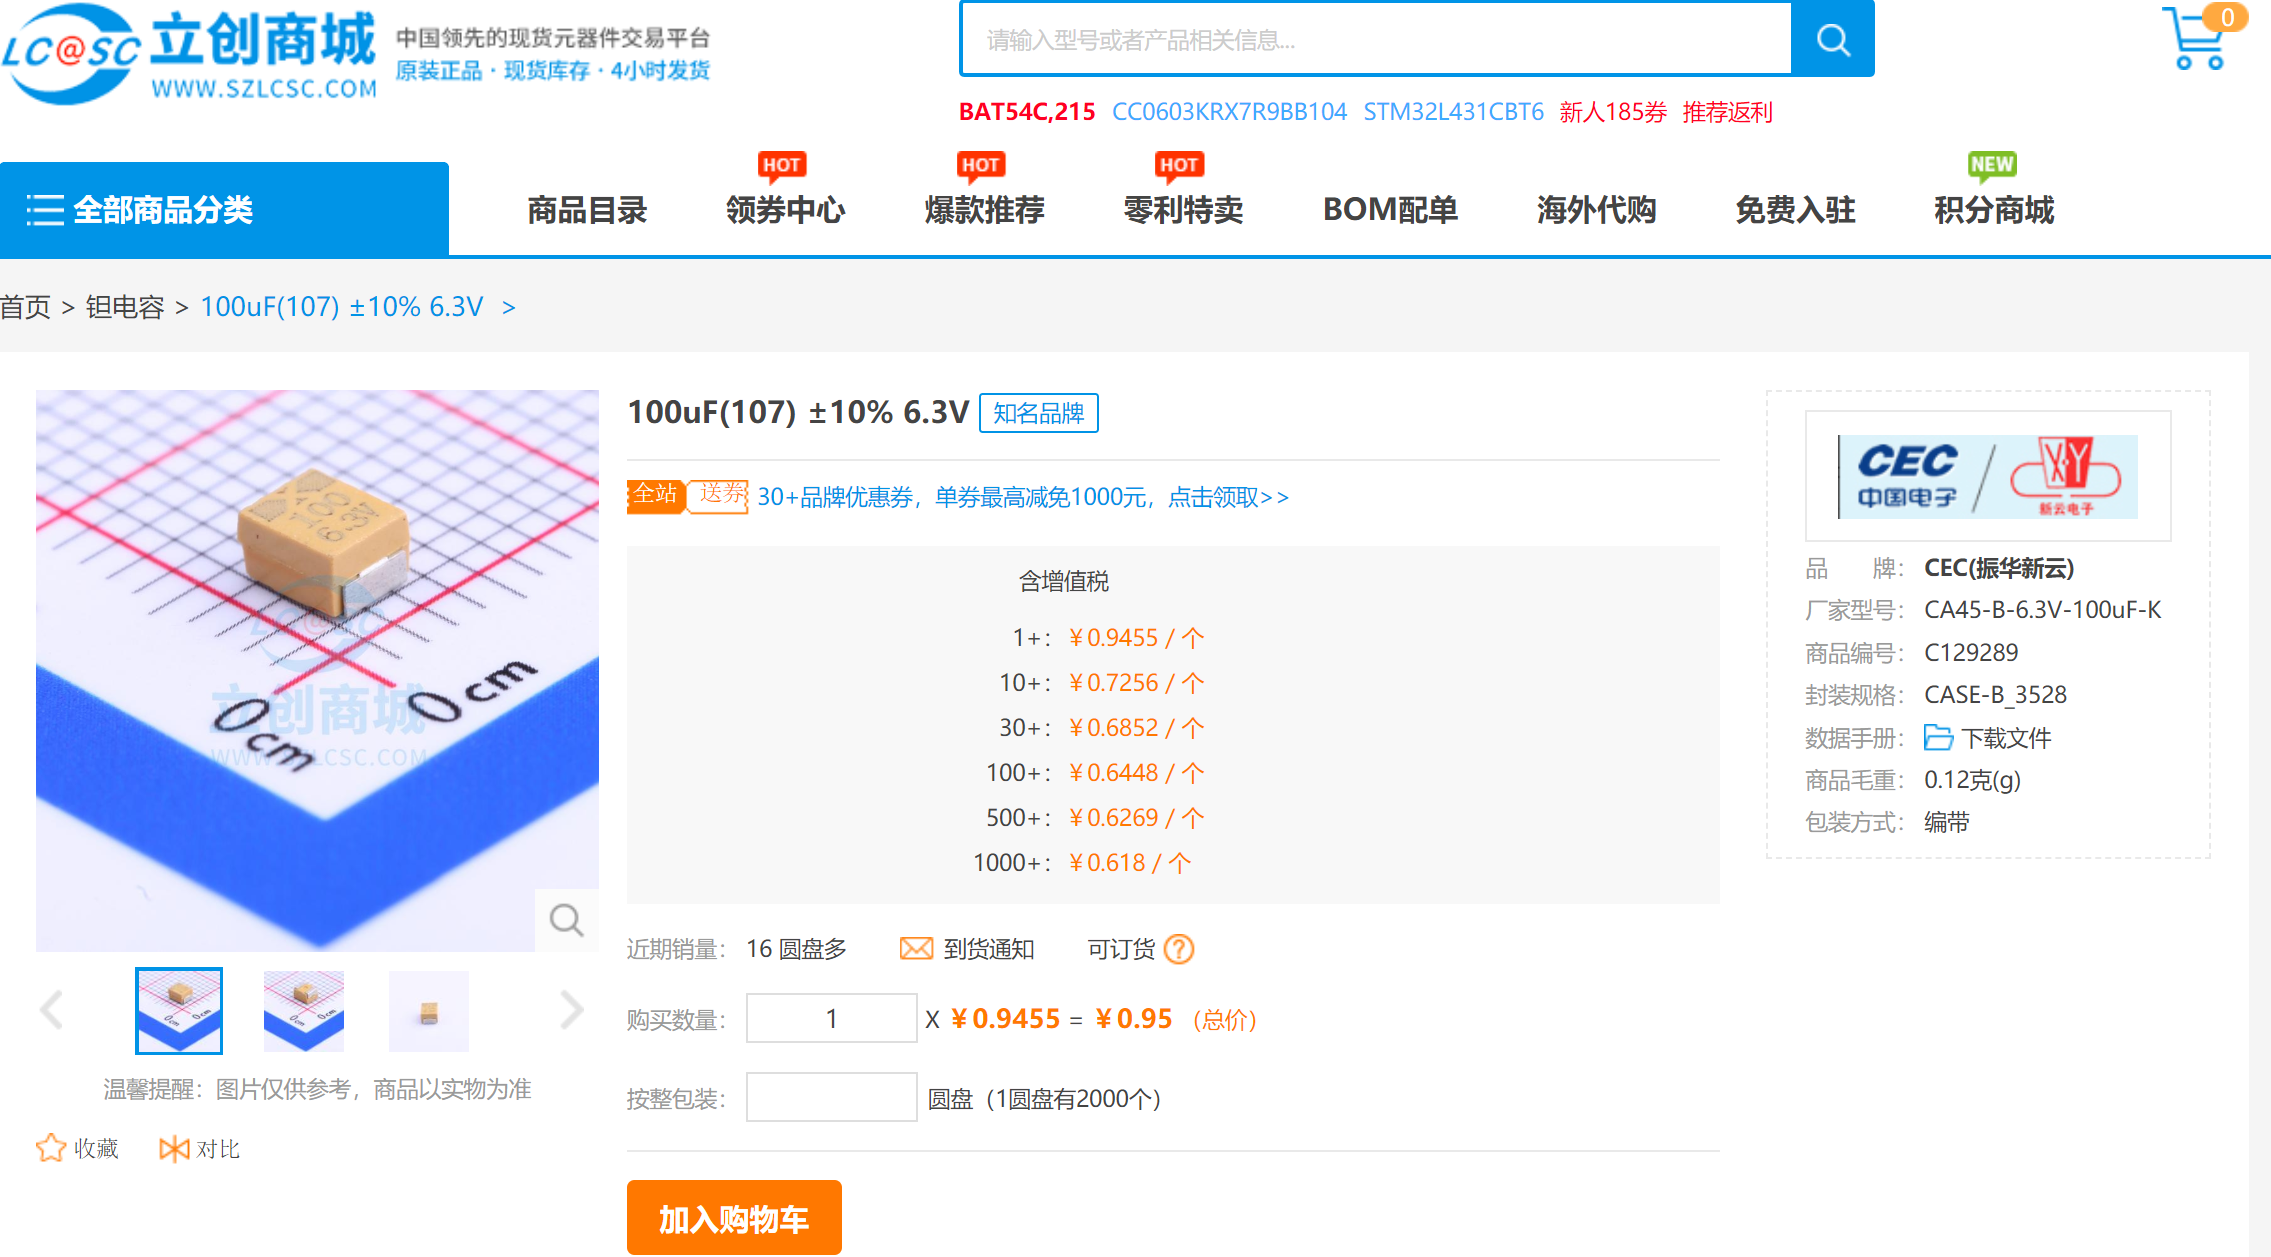
\includegraphics[width=\columnwidth]{DebugCapacitor3.png}
    \caption{钽电容的型号和耐压值}
    \label{fig:DebugCapacitor3}
\end{figure}

还有一块MCU芯片引脚弯了连在了一起,所以能烧程序但没有输出,试着能不能抢救,用指甲刀剪掉了空置的短路弯曲引脚,如图~\ref{fig:DebugShortCircuit},但是并没有解决问题,要用热风枪换芯片。

\begin{figure}[htbp]
    \centering
    \includegraphics[width=\columnwidth]{DebugShortCircuit.jpg}
    \caption{剪掉了空置的短路弯曲引脚的芯片}
    \label{fig:DebugShortCircuit}
\end{figure}

2020/4/23调试的第四块PCB的3号电机驱动电流参考电压一直是0V,更换了30k 50k电阻无果,3.3V输出正常,目测引脚没有异样短路,原因未知,先使用两个电机测试。